\usetikzlibrary{arrows.meta,calc}
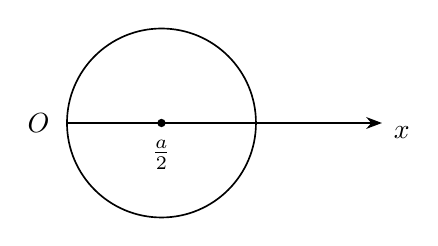
\begin{tikzpicture}[x=1cm,y=1cm,line width=.6pt,font=\normalsize,every node/.style={inner sep=0pt},>=Stealth]
\coordinate (O) at (0,0);
\coordinate (C) at (1.2,0);
\draw[->] (0,0)--(4.0,0) node[anchor=north west,inner sep=0pt,xshift=4pt,yshift=-1pt] {$x$};
\draw (1.2,0) circle[radius=1.2cm];
\fill (C) circle[radius=1.5pt];
\node[anchor=east,inner sep=0pt,xshift=-6pt] at (O) {$O$};
\node[anchor=north,inner sep=0pt,yshift=-6pt] at (C) {$\frac{a}{2}$};
\end{tikzpicture}
